% !TEX encoding = UTF-8
% !TEX TS-program = pdflatex
% !TEX root = ../Tesi.tex
% !TEX spellcheck = it-IT

\clearpage

\section{Attore arbitro}
%
% Figura: casi d'uso dell'attore arbitro
%
\begin{figure}[h]
	\centering
	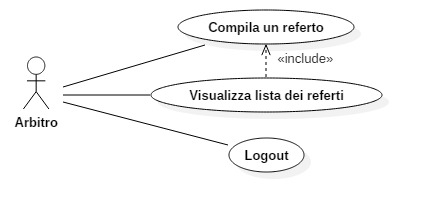
\includegraphics[width=0.7\textwidth]
	{immagini/uc-arbitro}
	
	\caption{Casi d'uso dell'attore arbitro}
\end{figure}


%
% Caso d'uso: Logout
%
\subsection{Caso d'uso: Logout}

\subsubsection*{Descrizione}
Questa funzionalità permette all'arbitro di uscire dalla sua pagina e di iniziare a navigare come utente pubblico.
Il pulsante di Logout è presente in ogni pagina dell'applicazione web, in alto a destra.

\subsubsection*{Attori coinvolti}
Arbitro, partecipazione attiva dell'attore verso il caso d'uso medesimo.

\subsubsection*{Pre-condizioni}
È richiesto l'accesso al sistema tramite la funzionalità di login.

\subsubsection*{Post-condizioni}
Termina la sessione di accesso al sistema in qualità di arbitro.

\subsubsection*{Flusso principale}

\begin{enumerate}
	
	\item
	L'arbitro seleziona nella pagina in cui si trova il pulsante di Logout;
	
	\item
	Il sistema scollega l'arbitro dalle pagine a lui riservate;
	
	\item
	Il sistema redireziona l'arbitro nella schermata di login e da quel momento può navigare come utente pubblico.
	
\end{enumerate}

\subsubsection*{Flussi alternativi}
Nel caso di operazione non riuscita si notifica all'arbitro il tipo di errore che si è verificato.

\subsection*{Diagramma delle attività}
Il diagramma delle attività per il caso d'uso ``Logout'' è illustrato nella figura \vref{ad-logout}.

%
% Caso d'uso: Visualizza lista dei referti
%
\subsection{Caso d'uso: Visualizza lista dei referti}

\subsubsection*{Descrizione}
Questa funzionalità permette all'arbitro di vedere tutti i referti che deve compilare o che ha già compilato.

\subsubsection*{Attori coinvolti}
Arbitro, partecipazione attiva dell'attore verso il caso d'uso medesimo.

\subsubsection*{Pre-condizioni}
È richiesto l'accesso al sistema come arbitro, tramite la funzionalità di login, in quanto solo lui ha il privilegio di poter visualizzare tale pagina.

\subsubsection*{Post-condizioni}
Nessuna post-condizione in quanto la visualizzazione dello dei referti non contribuisce a cambiare lo stato del sistema.

\subsubsection*{Flusso principale}

\begin{enumerate}
	
	\item
	L'arbitro seleziona la voce ``Nuovo Referto'' nella propria home page oppure seleziona la voce ``Referti'' nella pagina in cui si trova;
	
	\item
	Il sistema visualizza tutti i referti in ordine di id mostrandone: id del referto, nome del torneo, squadre sfidanti e data della partita. Il sistema, inoltre, visualizza per ogni referto un pulsante per compilarlo oppure visualizza ``Compilato'' se il referto è già stato compilato. 
	
\end{enumerate}

\subsubsection*{Flussi alternativi}
Nel caso di operazione non riuscita, si notifica all'arbitro il tipo di errore che si è verificato.


%
% Caso d'uso: Compila referto
%
\subsection{Caso d'uso: Compila referto}

\subsubsection*{Descrizione}
Questa funzionalità permette all'arbitro di compilare un referto che gli è stato assegnato relativo ad una partita.

\subsubsection*{Attori coinvolti}
Arbitro, partecipazione attiva dell'attore verso il caso d'uso medesimo.

Amministratore, partecipazione non attiva dell'attore verso il caso d'uso medesimo in quanto l'amministratore è responsabile solo della creazione della partita che l'arbitro dovrà dirigere.

Gestore squadra, partecipazione non attiva dell'attore verso il caso d'uso medesimo in quanto il gestore della squadra ha fornito la formazione della squadra per la partita a cui riferisce il referto.

\subsubsection*{Pre-condizioni}
È richiesto l'accesso al sistema come arbitro, tramite la funzionalità di login, in quanto solo lui ha il privilegio di poter compilare il referto di una partita. È richiesto che l'arbitro sia stato assegnato alla partita dall'amministratore. È necessario che entrambe le squadre abbiano fornito la formazione per la partita a cui fa riferimento il referto.

\subsubsection*{Post-condizioni}
Viene aggiornato lo stato sul database con l'aggiornamento del referto e viene aggiornata la classifica delle due squadre che hanno disputato l'incontro. In caso di torneo ad eliminazione diretta si provvede a qualificare al turno successivo la squadra che ha vinto.

\subsubsection*{Flusso principale}

\begin{enumerate}
	
	\item
	L'arbitro seleziona la voce ``Compila'' nella pagina di visualizzazione dei referti;
	
	\item
	Il sistema visualizza la pagina per l'inserimento dell'orario di inizio e l'orario di fine della partita;
	
	\item
	L'arbitro inserisce gli orari effettivi di inizio e fine della partita e successivamente seleziona la voce ``Conferma Orari'';
	
	\item
	Il sistema controlla i dati inseriti e se sono corretti visualizza le due formazioni con i giocatori di entrambe le squadre. Per ogni giocatore il sistema visualizza: foto del giocatore, numero maglia, nome e cognome del giocatore, campo per inserire il numero di goal effettuati e campo per inserire il numero di ammonizioni. Il sistema, inoltre, visualizza il numero di autogol effettuati per ciascuna squadra;
	
	\item
	L'arbitro inserisce i campi richiesti e conferma l'inserimento selezionando la voce ``Conferma'';
	
	\item
	Il sistema chiede conferma all'arbitro della compilazione del referto della partita. Se l'arbitro acconsente il sistema elabora i dati, altrimenti non avviene alcuna operazione e permette all'arbitro di modificare i dati inseriti;
	
\end{enumerate}

\subsubsection*{Flussi alternativi}
Nel caso di operazione non riuscita, si notifica all'arbitro il tipo di errore che si è verificato.

\subsection*{Diagramma delle attività}
Il diagramma delle attività per il caso d'uso ``Compila referto'' è illustrato nella figura \vref{ad-referto}.


%
% Figura: diagramma delle attività relativo alla compilazione di un referto
%
\begin{figure}[h]
	\centering
	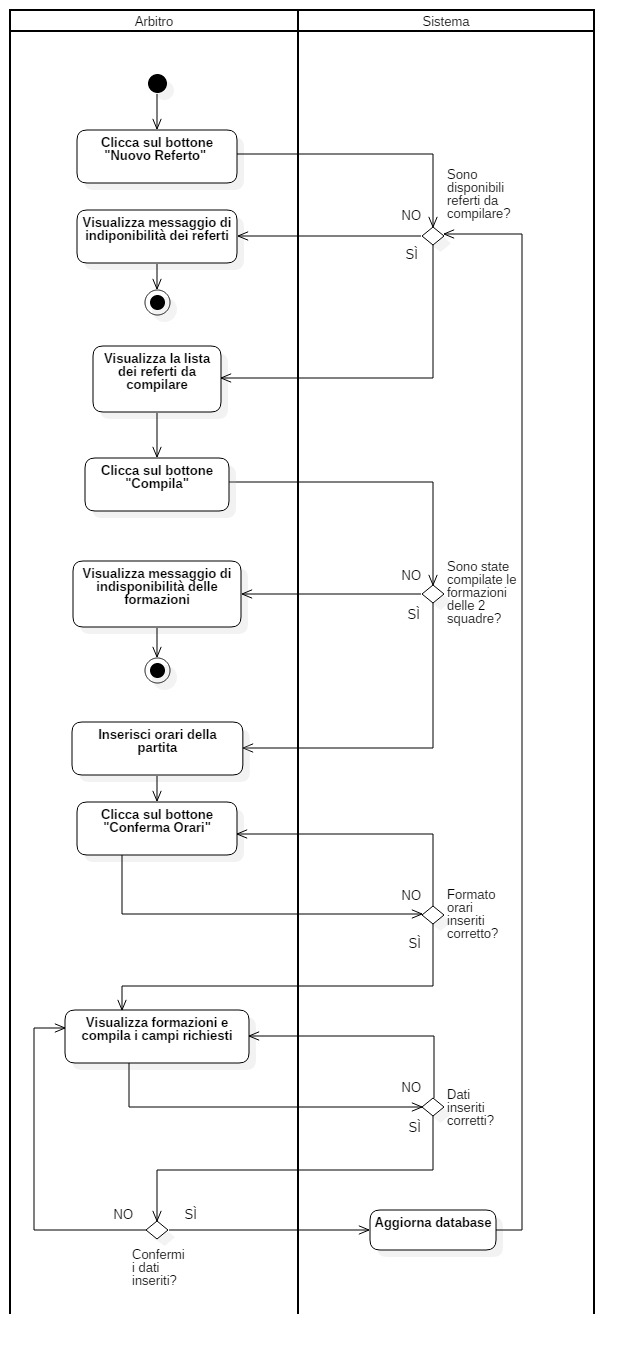
\includegraphics[width=0.8\textwidth]
	{immagini/ad-referto}
	
	\caption{Diagramma delle attività della compilazione di un referto}
	\label{ad-referto}
\end{figure}


%
% Figura: diagramma delle attività relativo al logout di un utente
%
\begin{figure}
	\centering
	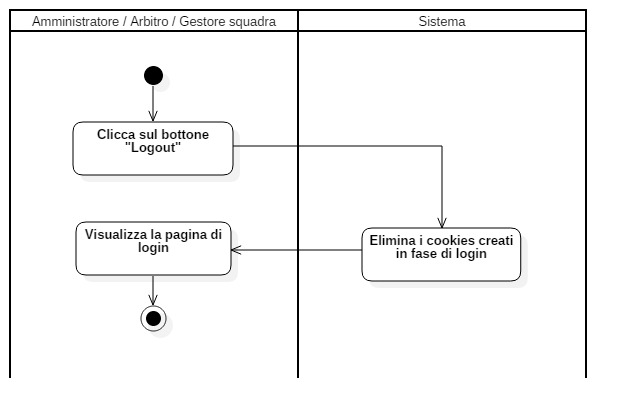
\includegraphics[width=0.8\textwidth]
	{immagini/ad-logout}
	
	\caption{Diagramma delle attività del logout di un utente}
	\label{ad-logout}
\end{figure}